\documentclass[
aps,
prl,
onecolumn,
amsmath,
amssymb,
superscriptaddress,
longbibliography
]{revtex4-2}

\usepackage{bm}
\usepackage{graphicx}
\usepackage{xcolor}
\usepackage[
colorlinks=true,
citecolor=blue!55!black,
urlcolor=blue!55!black,
linkcolor=blue!55!black
]{hyperref}

\graphicspath{{figs/}}
\setlength{\emergencystretch}{3em}

\newcommand{\bq}{\bm q}
\newcommand{\Szz}{S^{zz}}

\begin{document}

\title{
Supplemental Material for
``Roton-like Reconstruction of the Emergent Photon in Quantum Spin Ice''
}

\author{Zhengbang Zhou}
\affiliation{
Department of Physics, University of Toronto,
Toronto, Ontario M5S 1A7, Canada
}

\author{Yong Baek Kim}
\affiliation{
Department of Physics, University of Toronto,
Toronto, Ontario M5S 1A7, Canada
}

\maketitle

% ================================================================
\section{Theoretical response and relation to neutron scattering}
\label{sec:observable}
% ================================================================

The quantity calculated in the Letter is the zero-temperature,
sublattice-summed longitudinal pseudospin correlation function
\begin{equation}
\Szz(\bq,\omega)
=
\frac{1}{N}
\sum_{\mu,n}
\left|
\langle n|S_\mu^z(\bq)|0\rangle
\right|^2
\delta(\omega-\omega_n),
\label{eq:szz_supp}
\end{equation}
where
\begin{equation}
S_\mu^z(\bq)
=
\sum_{i\in\mu}
e^{-i\bq\cdot\bm r_i}S_i^z
\end{equation}
and $\mu$ runs over the four pyrochlore sublattices.

Inside the spin-ice manifold, $S_i^z$ is the component of the
pseudospin along the local $\langle111\rangle$ easy axis and equals
the emergent electric field,
\begin{equation}
E_i=S_i^z .
\end{equation}

Every quoted spectral fraction is normalized at fixed momentum:
\begin{equation}
Z_n(\bq)
=
\frac{
\sum_\mu
|\langle n|S_\mu^z(\bq)|0\rangle|^2
}{
\sum_{m,\mu}
|\langle m|S_\mu^z(\bq)|0\rangle|^2
}.
\end{equation}

Equation~(\ref{eq:szz_supp}) is not by itself the laboratory neutron
cross section.
A material-specific magnetic cross section contains the ionic form
factor, the $g$ tensor, the rotation between the four local
$\langle111\rangle$ frames and the laboratory frame, the neutron
polarization tensor
\begin{equation}
\delta_{\alpha\beta}
-
\hat q_\alpha\hat q_\beta,
\end{equation}
and coherent interference between different sublattices.

Schematically,
\begin{equation}
I(\bq,\omega)
\propto
\sum_{\mu\nu}
{\cal F}_{\mu\nu}(\bq)
S_{\mu\nu}^{zz}(\bq,\omega),
\end{equation}
where
\begin{equation}
S_{\mu\nu}^{zz}(\bq,\omega)
=
\sum_n
\langle0|
S_\mu^z(-\bq)
|n\rangle
\langle n|
S_\nu^z(\bq)
|0\rangle
\delta(\omega-\omega_n).
\end{equation}

The $50$--$54\%$ low-mode fractions quoted in the Letter therefore
refer strictly to the sublattice-summed pseudospin response.
They are not universal neutron-intensity fractions.
A material-specific prediction requires applying the coherent
projection appropriate to the material's local axes and $g$ tensor.

% ================================================================
\section{Contractible ring terms and finite clusters}
\label{sec:clusters}
% ================================================================

The Hamiltonian is
\begin{equation}
H
=
-K\sum_p
\left(
W_p+W_p^\dagger
\right),
\qquad
W_p
=
S_1^+S_2^-S_3^+S_4^-S_5^+S_6^- .
\label{eq:ring_supp}
\end{equation}

On a periodic finite cluster, six-site closed paths come in two
classes:
elementary contractible hexagons corresponding to plaquettes of the
infinite pyrochlore lattice, and loops that close only by winding
around the torus.
The latter are not local plaquettes of the thermodynamic Hamiltonian.
We therefore compute the winding vector of every six-cycle and retain
only zero-winding elementary hexagons.

For every cluster used in the Letter, the retained Hamiltonian has the
full lattice density of elementary rings.

The principal finite clusters are
\begin{center}
\begin{tabular}{lrrrr}
\hline\hline
&
$2\times2\times3$
&
$2\times2\times4$
&
$2\times3\times3$
&
$2\times3\times4$
\\
\hline
sites
&
48&64&72&96
\\
ice configurations
&
$87\,546$
&
$2\,756\,394$
&
$12\,846\,186$
&
$2\,007\,260\,562$
\\
spectral sector dimension
&
$9\,104$
&
$249\,180$
&
$973\,008$
&
$146\,758\,352$
\\
\hline\hline
\end{tabular}
\end{center}

The commonly used 16- and 32-site pyrochlore clusters are
pathological for the present dynamical question.
On the 32-site cell every configuration in the connected zero-flux
sector has exactly eight flippable hexagons.
The equal-amplitude state is consequently an exact eigenstate and the
spectrum becomes artificially integer-like.
On the 16-site cluster only six transport sectors possess nontrivial
ring dynamics.
We therefore begin with 48 sites.

Varying cluster shape at fixed spin number is also not a clean option.
At these sizes, alternative thin tori containing an $L$-type momentum
lose a substantial fraction of the contractible elementary rings.
For example, the $1\times3\times4$ 48-site cell contains only 24
contractible hexagons.
Keeping only those terms produces a Hamiltonian with half the ring
density and therefore a different microscopic model.
The finite-size analysis consequently uses the sequence of admissible
clusters listed above.

% ================================================================
\section{Winding sectors}
\label{sec:winding}
% ================================================================

The ring Hamiltonian conserves topological winding polarization.
Configurations are assigned an exact integer key derived from
\begin{equation}
\bm P
=
\sum_i
\left(n_i-\frac12\right)\bm r_i .
\end{equation}

On the 48-site cluster all winding sectors can be enumerated
explicitly.
The global ground state lies in the sector of dimension $9104$ used
for complete diagonalization.

On 72 sites the zero-polarization sector is empty.
The ground states instead form a degenerate $\pm\bm P$ pair of
nonzero-polarization sectors, each of dimension
\begin{equation}
973\,008
\end{equation}
and energy
\begin{equation}
E_0=-14.80971536K .
\end{equation}
The identification is verified by independent diagonalization of the
largest candidate sectors.

% ================================================================
% IMPORTANT BEFORE SUBMISSION:
%
% The current 96-site calculation explicitly diagonalizes the three
% largest candidate winding sectors and finds the lowest among them.
% It does not rigorously exclude every smaller sector.
%
% Replace this note with either
%
% (i) a complete/exhaustive certification,
% (ii) a rigorous lower-bound argument,
% or
% (iii) wording throughout the paper that calls this "the lowest
%       sector among those tested."
%
% Sector dimension itself is not a variational criterion.
% ================================================================

% ================================================================
\section{Enumeration and Lanczos spectroscopy}
\label{sec:methods}
% ================================================================

Ice configurations are enumerated exactly by assigning spins
sequentially and backtracking whenever a tetrahedron would acquire
three spins of either sign.
For every elementary hexagon, a bit mask and its two alternating
flippable patterns identify the states connected by the ring
Hamiltonian.

On 48 sites the $9104$-dimensional sector is diagonalized completely
with a dense symmetric eigensolver.
All eigenvalues and eigenvectors are therefore available.

At 64 sites the sector dimension is $249\,180$.
The dynamical response is obtained through Lanczos continued
fractions seeded independently by
\begin{equation}
S_\mu^z(\bq)|0\rangle .
\end{equation}
The 64-site calculation uses full reorthogonalization.

Going beyond 64 spins requires replacing the single-word bit
representation.
For 72 and 96 sites, each configuration is represented by a pair of
64-bit words.
All masking, flipping, sorting, and exact lookup operations are
implemented on the word pair.

The two-word pipeline is validated on the 48-site cluster, where it
reproduces
\begin{align}
E_0&=-10.55601176K,\\
S(L)&=0.37036,
\end{align}
and the principal $L$ energies
\begin{equation}
1.0235K,\qquad1.7303K
\end{equation}
exactly relative to the single-word implementation.

On 96 sites the complete ice manifold contains
\begin{equation}
2\,007\,260\,562
\end{equation}
configurations.
It is enumerated using a vectorized frontier algorithm that imposes
one tetrahedron constraint at a time and branches the frontier into
independent seeds.
The spectral sector contains
\begin{equation}
146\,758\,352
\end{equation}
basis states and approximately
\begin{equation}
2.7\times10^9
\end{equation}
nonzero Hamiltonian matrix elements.

The continued-fraction calculation uses real Lanczos separately on
the real and imaginary parts of the probe.
This is exact for a real symmetric Hamiltonian and reduces Krylov
storage.
On the 72-site cluster, 120 real iterations reproduce the
250-iteration complex calculation to every printed digit.

Degenerate eigenvalues are grouped within
\begin{equation}
10^{-8}K
\end{equation}
and their spectral weights summed before branch weights are quoted.
Only the total weight of a degenerate multiplet is basis invariant.

Momentum labels are certified by explicit translation projectors
rather than inferred from an ordering of the numerical eigenstates.

Three exact gates are applied throughout:
\begin{enumerate}
\item the plaquette-energy identity
\begin{equation}
\sum_p
\langle
W_p+W_p^\dagger
\rangle
=
-\frac{E_0}{K},
\end{equation}
\item agreement of the spectral first moment with the exact
double-commutator result, and
\item the gauge identity
\begin{equation}
Cd_0=0
\end{equation}
for the lattice curl.
\end{enumerate}

% ================================================================
% REQUIRED 96-SITE CONVERGENCE ADDITION
%
% Add a table/figure such as
%
% m       omega_low       Z_low       omega_high      residual
% 60      ...
% 80      ...
% 100     ...
% 120     ...
% 160     ...
%
% and state the orthogonalization strategy at 96 sites.
%
% The equal-time sum rule is not by itself sufficient to certify
% convergence of individual spectral poles.
% ================================================================

% ================================================================
\section{Gaussian lattice electrodynamics}
\label{sec:gaussian}
% ================================================================

Every comparison with a ``Gaussian photon'' is made using the lattice
curl on the same finite torus as the microscopic calculation.

Write
\begin{equation}
B_p
=
\sum_\ell C_{p\ell}A_\ell,
\end{equation}
where $C$ is the alternating lattice curl.
Expanding the compact magnetic energy to quadratic order and
introducing the electric stiffness gives
\begin{equation}
H_G
=
\frac{U}{2}
\sum_\ell E_\ell^2
+
K\sum_p B_p^2,
\qquad
[A_\ell,E_{\ell'}]
=
i\delta_{\ell\ell'} .
\label{eq:hg}
\end{equation}

At fixed momentum, the normal-mode frequencies are determined by the
nonzero singular values of the curl block,
\begin{equation}
\omega_\lambda(\bq)
=
\sqrt{2UK}\,
\sigma_\lambda(\bq).
\label{eq:gaussian}
\end{equation}

The construction satisfies three checks:
\begin{enumerate}
\item gauge invariance,
\begin{equation}
Cd_0=0
\end{equation}
to machine precision;
\item exactly two nonzero singular values for every
$\bq\neq\Gamma$ and none at $\Gamma$;
\item orthonormality and completeness of the Bloch basis.
\end{enumerate}

The pure ring Hamiltonian contains no independent bare value of $U$,
so one overall scale must be inferred from the interacting spectrum.
A single linear least-squares fit gives
\begin{equation}
\sqrt{2UK}=0.5868K.
\end{equation}
At $L$ this gives
\begin{equation}
\omega_G(L)=2.03K.
\end{equation}

The fitted curve is used only to quantify the magnitude of the
reconstruction and to compare momentum dependence.
The scale-free branch ratio and spectral-weight fractions quoted in
the Letter do not depend on this fit.

% ================================================================
\section{Basis-invariant transverse-channel resolution}
\label{sec:polarization}
% ================================================================

At each momentum the electric-field probe spans the four-dimensional
sublattice space.
The lattice curl has rank two, leaving a two-dimensional transverse
physical subspace.
The residual weight in the remaining longitudinal directions is less
than
\begin{equation}
10^{-31}
\end{equation}
relative to $S(\bq)$.

The two Gaussian singular values are exactly degenerate, so an
individual transverse basis is defined only up to a rotation.
Statements assigning a level to a particular arbitrarily chosen
Gaussian polarization are therefore not invariant.

For a level of multiplicity $m$, let $A_n$ be the
$m\times2$ matrix of amplitudes in any orthonormal transverse basis.
We define
\begin{equation}
M_n
=
A_n^\dagger A_n .
\end{equation}
The polarization purity is
\begin{equation}
{\cal P}_n
=
\frac{
\mathrm{tr}\,M_n^2
}{
(\mathrm{tr}\,M_n)^2
},
\end{equation}
and the normalized overlap between two levels is
\begin{equation}
{\cal O}_{AB}
=
\frac{
\mathrm{tr}(M_AM_B)
}{
\mathrm{tr}M_A\,
\mathrm{tr}M_B
}.
\end{equation}
Both quantities are invariant under rotations of the transverse
basis.

Representative 48-site results are
\begin{center}
\begin{tabular}{lrrrr}
\hline\hline
$\bq$
&
$\omega_1/K$
&
$\omega_2/K$
&
splitting
&
overlap
\\
\hline
$(\frac13,\frac13,\frac13)$
&1.895&1.980&0.044&$2\times10^{-28}$
\\
$(\frac13,\frac13,\frac23)$
&1.744&2.069&0.171&$10^{-29}$
\\
$(\frac16,\frac16,\frac56)$
&2.533&2.687&0.059&$4\times10^{-2}$
\\
$L$
&1.024&1.730&0.513&$3\times10^{-3}$
\\
$X$
&2.235&3.423&0.420&$10^{-31}$
\\
\hline\hline
\end{tabular}
\end{center}

The two brightest levels are nearly orthogonal directions within the
two-dimensional transverse probe space.
We use this result to speak operationally of two transverse
$S^z$-active branches.
The polarization geometry by itself is not taken as proof of an
adiabatic quasiparticle ancestry.

% ================================================================
\section{Exact first moment and Feynman ratio}
\label{sec:feynman}
% ================================================================

The first spectral moment is
\begin{equation}
f_1(\bq)
=
\frac{1}{2N}
\sum_\mu
\langle0|
[
S_\mu^z(-\bq),
[
H,S_\mu^z(\bq)
]
]
|0\rangle .
\end{equation}
For the ring Hamiltonian this reduces exactly to
\begin{equation}
f_1(\bq)
=
\frac{K}{2N}
\sum_p
\left\langle
W_p+W_p^\dagger
\right\rangle
\sum_\mu
\left|
g_p^\mu(\bq)
\right|^2 .
\label{eq:f1_supp}
\end{equation}

The zeroth moment is
\begin{equation}
S(\bq)
=
\int d\omega\,
\Szz(\bq,\omega),
\end{equation}
so the normalized state proportional to
$S^z(\bq)|0\rangle$ has variational energy
\begin{equation}
\omega_{\rm SMA}(\bq)
=
\frac{f_1(\bq)}{S(\bq)}.
\end{equation}

This ratio is identically the spectral centroid.
Its value after a spectrum has been calculated is therefore not
independent evidence for a low pole.
The nontrivial tests used in the Letter are instead the predictions
made using the ground-state ratio before the corresponding excited
states are calculated.

% ================================================================
\section{Geometry and the interacting enhancement of $S(L)$}
\label{sec:geometry}
% ================================================================

The oscillator strength has an especially transparent geometric
structure.
If a hexagon lies inside a wavefront of the electric-field
oscillation, the alternating loop integral vanishes identically and
the plaquette contributes nothing to Eq.~(\ref{eq:f1_supp}).

At
\begin{equation}
L\parallel[111],
\end{equation}
one of the four hexagon families lies in the wavefronts.
On the 48-site cluster the family-resolved geometric factors are
\begin{equation}
(96,96,96,0)_L,
\end{equation}
compared with
\begin{equation}
(96,96,96,96)_X .
\end{equation}

The reduction in the pure geometric factor is therefore exactly
$3/4$.
The reduction of $f_1$ itself is not exactly $3/4$ because the
ground-state plaquette coherences are not perfectly uniform on an
anisotropic cluster.
Numerically,
\begin{equation}
\frac{f_1(L)}{f_1(X)}
=
\frac{0.684}{0.880}
=
0.777.
\end{equation}

The geometric cancellation alone does not generate the anomaly.
At the shortest sampled momentum along $[111]$, one family is also
exactly dark, but the dominant level remains near the Gaussian
photon.

The second ingredient is the interacting equal-time structure factor.
On 48 sites,
\begin{equation}
S(L)=0.370
\end{equation}
for the quantum ground state, compared with
\begin{equation}
S_{\rm EA}(L)=0.297
\end{equation}
for the equal-amplitude superposition over the same 9104
configurations.

A classical loop-update calculation on a 2048-site ice manifold gives
\begin{align}
S(L)&=0.2488(67),\\
S(X)&=0.2538(73),\\
S(W)&=0.2475(52),\\
S(K)&=0.2467(46).
\end{align}
Within statistical precision the classical zone-boundary structure
factor is essentially flat.
The enhancement near $L$ is therefore generated predominantly by the
interacting quantum amplitudes at the physical ring point.

The 72-site soft-valley momentum
\begin{equation}
\bq_v
=
\left(
\frac16,\frac12,\frac12
\right)
\end{equation}
has geometric family weights
\begin{equation}
(36,144,144,108),
\end{equation}
so no family is exactly dark.
Nevertheless its enhanced structure factor produces an $f_1/S$
within $0.9\%$ of the $L$ value, and the two reconstructed levels are
within $0.7\%$ of one another.

% ================================================================
\section{Rokhsar--Kivelson deformation}
\label{sec:rk}
% ================================================================

We use the standard RK extension
\begin{equation}
H(V)
=
-K\sum_p
\left(
W_p+W_p^\dagger
\right)
+
V\sum_p n_p^{\rm flip},
\label{eq:rk_supp}
\end{equation}
where $n_p^{\rm flip}$ projects onto a flippable alternating
hexagon.

Our sign convention is such that
\begin{equation}
V>0
\end{equation}
penalizes flippability,
\begin{equation}
V<0
\end{equation}
rewards it, and the exactly solvable RK point is at
\begin{equation}
V=+K.
\end{equation}

For state characterization we use only the derivative at the
physical ring point $V=0$.
Hellmann--Feynman gives
\begin{equation}
\frac{d\omega_n}{dV}
=
\left\langle n\left|
N_{\rm flip}
\right|n\right\rangle
-
\left\langle0\left|
N_{\rm flip}
\right|0\right\rangle ,
\qquad
N_{\rm flip}
=
\sum_p n_p^{\rm flip}.
\label{eq:hf}
\end{equation}

Thus $d\omega_n/dV$ is an exact state-resolved measure of the
difference in the number of flippable plaquettes between an
excitation and the ground state.

At 48 sites the reconstructed $L$ level has
\begin{equation}
\frac{d\omega_{\rm low}}{dV}
=
+0.339.
\end{equation}
The upper $L$ level responds with the opposite sign.

Across the four finite sizes the reconstructed levels have
\begin{equation}
+0.339,\quad
+0.338,\quad
+0.134,\quad
+0.259 .
\end{equation}
The sign remains positive, but the magnitude is not size stable.
We therefore do not use the census as the primary discriminator.

% ================================================================
\subsection{Exact census sum rule}
% ================================================================

The operator $N_{\rm flip}$ is diagonal in the configuration basis.
Every flippable hexagon generates exactly one off-diagonal
ring-connected state.
Consequently
\begin{equation}
\mathrm{Tr}\,N_{\rm flip}
=
\mathrm{nnz}(H),
\end{equation}
where $\mathrm{nnz}(H)$ denotes the number of nonzero off-diagonal
matrix elements, with the same counting convention.

Averaging Eq.~(\ref{eq:hf}) over the complete spectrum of a sector of
dimension $D$ gives
\begin{equation}
\frac{1}{D}
\sum_n
\frac{d\omega_n}{dV}
=
\frac{
\mathrm{nnz}(H)
}{D}
-
\langle0|
N_{\rm flip}
|0\rangle .
\label{eq:census_sum}
\end{equation}

On the 48-site sector,
\begin{equation}
\frac{1}{D}
\sum_n
\frac{d\omega_n}{dV}
=
-0.9139,
\end{equation}
and the direct average over all 9104 eigenstates reproduces this value
to $10^{-14}$.

Excitations therefore lose flippability on average.
There is no sign theorem for an individual eigenstate.
Of the 9104 eigenstates,
\begin{equation}
58
\end{equation}
have positive census and
\begin{equation}
20
\end{equation}
exceed $+0.20$.
The reconstructed $L$ state at $+0.339$ lies in the extreme positive
tail but is not unique.

The cleaner census result is the within-cluster comparison.
The 64- and 96-site clusters each contain two inequivalent $L$-type
classes at identical $|\bq|$ and identical Gaussian energy.
Their censuses are
\begin{align}
64:\quad&
+0.338
\quad{\rm versus}\quad
-0.166,\\
96:\quad&
+0.259
\quad{\rm versus}\quad
-0.02,\,-0.09 .
\end{align}
The classes that reconstruct and those that do not therefore respond
with opposite signs to the same microscopic flippability probe.

% ================================================================
\subsection{Finite RK trajectory}
% ================================================================

For completeness we also follow the reconstructed level over a finite
range of $V$.
Biasing toward more flippable configurations, $V<0$, increases
$S(L)$ and softens the low level from approximately
\begin{equation}
1.02K
\end{equation}
to
\begin{equation}
0.73K
\end{equation}
over the range studied, while $f_1(L)$ changes by less than one
percent.

This evolution is consistent with the Feynman-ratio description:
the softening accompanies an enhancement of the equal-time
fluctuation while the oscillator strength is nearly unchanged.
We do not interpret the deformation as establishing a temporal or
causal ordering between ground- and excited-state quantities.

% ================================================================
\section{Variational relaxation of the reconstructed state}
\label{sec:variational}
% ================================================================

The sublattice-resolved probe vectors
\begin{equation}
S_\mu^z(L)|0\rangle
\end{equation}
span the transverse electric-field trial space.
The lowest energy in this space on the 48-site cluster is
\begin{equation}
1.450K.
\end{equation}

A systematic variational improvement converges rapidly:
\begin{equation}
1.450
\rightarrow
1.074
\rightarrow
1.034
\rightarrow
1.026K,
\end{equation}
compared with the exact eigenvalue
\begin{equation}
1.024K.
\end{equation}
Thus the reconstructed state is reached in a small collective
subspace generated from the physical probe.

The fractional recovery relative to the bare optimized electric-field
state is
\begin{equation}
\frac{
\omega_{\rm bare}
-
\omega_{\rm exact}
}{
\omega_{\rm bare}
}
=
29\%
\end{equation}
on 48 sites.
The corresponding values on 48, 64, and 72 sites are
\begin{equation}
29\%,\qquad
32\%,\qquad
28\%.
\end{equation}

The identity of the state reached by this construction is itself a
measured quantity, and it is what ties the Feynman construction to
the lower branch specifically. The squared overlap of the
ground-state-projected single-mode state with the lower-branch
multiplet is
\begin{equation}
0.88,\qquad
0.87,\qquad
0.86
\end{equation}
on the 48-, 64-, and 72-site clusters; the state couples to the upper
branch only through the orthogonal transverse channel. The Feynman
(density-wave) construction therefore produces the lower branch, not
the upper one, at every size at which the comparison can be made.

% ================================================================
\section{Basis-invariant plaquette decomposition}
\label{sec:backflow}
% ================================================================

Because the ring term is the entire nonconstant Hamiltonian in the
ice manifold, every excitation energy decomposes exactly into
plaquette contributions:
\begin{equation}
\omega_n
=
-K
\sum_p
\left[
\langle n|
W_p+W_p^\dagger
|n\rangle
-
\langle0|
W_p+W_p^\dagger
|0\rangle
\right].
\label{eq:edecomp}
\end{equation}

Grouping plaquettes into the four $\langle111\rangle$ orientation
families gives a complete four-term decomposition.

The exact low level is degenerate.
Expectation values in an arbitrary basis of this multiplet are
therefore not physically invariant.
We choose the normalized projection of the physical $S^z$ probe onto
the degenerate multiplet.
This state is basis independent.
An alternative alignment to the optimized single-mode state gives
per-family values identical to four decimals.

The resulting decomposition is
\begin{center}
\begin{tabular}{lrrr}
\hline\hline
&48&64&72\\
\hline
single-mode energy
&1.450&1.412&1.481\\
exact low level
&1.024&0.954&1.068\\
recovery
&29\%&32\%&28\%\\
\hline
relief, family 1
&$+0.080$&$+0.040$&$+0.276$\\
relief, family 2
&$-0.064$&$-0.036$&$+0.002$\\
relief, family 3
&$+0.088^\star$&$+0.227$&$+0.002$\\
relief, family 4
&$+0.322$&$+0.227$&$+0.133^\star$\\
\hline
dark-family share
&21\%&9\%&32\%\\
\hline\hline
\end{tabular}
\end{center}
where $\star$ denotes the geometrically dark family for the
corresponding cluster.

The $28$--$32\%$ relaxation is stable across the three sizes.
It is strongly family selective, but it is not concentrated in the
geometrically dark family.

An earlier analysis obtained a $71\%$ dark-family contribution by
evaluating an arbitrary member of the degenerate multiplet.
That result is basis dependent and is withdrawn.
The corrected conclusion is a robust, family-selective reorganization
of ring coherence with a dark-family contribution of $9$--$32\%$.

% ================================================================
\section{Few-photon kinematics}
\label{sec:kinematics}
% ================================================================

Global spin reversal is an exact symmetry of the ring Hamiltonian.
For an even ground state the linear $S^z$ probe is odd and therefore
couples only to odd-parity eigenstates.
In gauge language this is charge conjugation, under which a state
containing $n$ weakly defined photons has parity
\begin{equation}
(-1)^n .
\end{equation}

Parity excludes even photon number but does not exclude three-photon
states.
We therefore minimize the energy of finite-volume Gaussian photon
partitions with total momentum $L$.

On the 48-site torus the resulting thresholds are
\begin{align}
\omega_L^{(1)}&=2.03K,\\
\omega_L^{(2)}&=4.03K,\\
\omega_L^{(3)}&=5.55K.
\end{align}

The reconstructed level lies at
\begin{equation}
1.02K,
\end{equation}
more than a factor of five below the weakly renormalized Gaussian
three-photon threshold.

This rules out an interpretation in terms of a few weakly interacting
Gaussian photons on the finite clusters.
Because the Letter itself establishes order-one interactions at the
zone boundary, the calculation is not a theorem excluding
multiparticle states formed from strongly renormalized constituents
in the thermodynamic theory.

% ================================================================
\section{Off-pole spectral weight and complementary probes}
\label{sec:offpole}
% ================================================================

Beyond the two dominant transverse branches,
\begin{equation}
16\%\text{--}38\%
\end{equation}
of the 48-site $S^z$ spectral weight resides in higher levels absent
from the Gaussian one-photon theory.
The off-pole fraction is smallest at the shortest accessible
momenta, consistent with recovery of the infrared photon.

Spin-reversal parity gives a clean separation of probe channels.
Numerically, every even state carries linear $S^z$ weight below
\begin{equation}
10^{-28}.
\end{equation}
Bilinear operators can instead couple to the even sector, including
two-particle channels, and can be accessed by probes such as Raman
scattering or ultrasound \cite{Fu2017,Simon2022}.
Magnetization probes such as neutron scattering and stray-field noise
belong to the odd channel \cite{Naik2026}.

\begin{figure}[t]
\centering
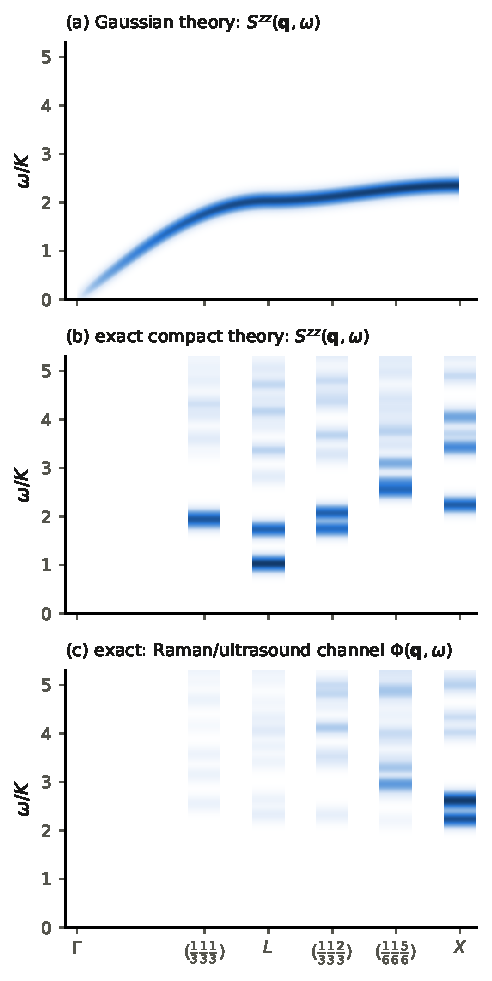
\includegraphics[width=0.90\textwidth]{fig_maps.pdf}
\caption{
Simulated spectra along $\Gamma$--$L$--$X$ for the 48-site cluster,
with display broadening $\eta=0.08K$.
(a) Gaussian one-photon response.
(b) Exact odd-parity $S^z$ response.
(c) Complementary even-parity response accessible to bilinear probes.
}
\label{fig:channels}
\end{figure}

% ================================================================
\section{Green's-function Monte Carlo}
\label{sec:gfmc}
% ================================================================

The ring Hamiltonian is stoquastic in the ice basis:
its diagonal matrix elements vanish and every nonzero off-diagonal
element is $-K$.
A power method with
\begin{equation}
\Lambda-H
\end{equation}
therefore converges to the ground state with nonnegative amplitudes.

We use the equal-amplitude trial state
\begin{equation}
|\Psi_T\rangle
=
\sum_x|x\rangle .
\end{equation}
Population control is performed by comb reconfiguration at fixed
walker number.

For diagonal observables such as $S(\bq)$, the mixed distribution
$\Psi_0\Psi_T$ is converted to the pure distribution
$|\Psi_0|^2$ by forward walking.
An observable measured at time $t$ is weighted by the number of
descendants retained by the walker after a projection time $T$.

Convergence is benchmarked on the exactly diagonalized 48-site
cluster using
\begin{equation}
256\text{--}2048
\end{equation}
walkers and
\begin{equation}
T=20\text{--}160.
\end{equation}
At $T=20$, the forward-walking estimate of $S(L)$ is biased low by
approximately $0.7\%$.
For
\begin{equation}
T\ge40
\end{equation}
the values fluctuate around the exact result
\begin{equation}
S(L)=0.370365
\end{equation}
within statistical errors.
Production runs use
\begin{equation}
T=80.
\end{equation}

The mixed-estimator energies exhibit a residual population-control
bias of approximately
\begin{equation}
1.5\times10^{-4}
\end{equation}
in relative units, independent of walker number over the tested
range.
This is two orders of magnitude below the energy differences used in
the analysis.

Initialization requires care because sublattice-uniform ice
configurations are frozen under the ring dynamics.
Seeds are randomized using worm-constructed loop flips that first
reduce the integer polarization and subsequently preserve the minimal
reachable polarization exactly.

Every production calculation is gated against exact diagonalization.
On 48 sites,
\begin{equation}
E_0=-10.556012K
\end{equation}
is reproduced within $0.5\sigma$, and
\begin{equation}
S(L)=0.370365
\end{equation}
is reproduced to every printed digit.

On 72 sites the method reproduces
\begin{equation}
E_0/N=-0.205690K
\end{equation}
within $1.8\sigma$ in the correct nonzero-polarization ground sector.

Production calculations use 1024 walkers and
$30\,000$--$60\,000$ propagation steps.
Statistical uncertainties are estimated from 16 bins.

On cubic supercells every hexagon is symmetry equivalent.
The exact identity
\begin{equation}
\sum_p
\langle
W_p+W_p^\dagger
\rangle
=
-\frac{E_0}{K}
\end{equation}
therefore fixes the uniform plaquette coherence directly from the
ground-state energy.
The remaining momentum dependence of $f_1$ is exact lattice geometry.

The complete momentum grids contain 216 momenta on the 864-site
$6^3$ cell and 512 momenta on the 2048-site $8^3$ cell.

% ================================================================
\section{Large-system centroid landscape}
\label{sec:thermo}

\begin{figure}[t]
\centering
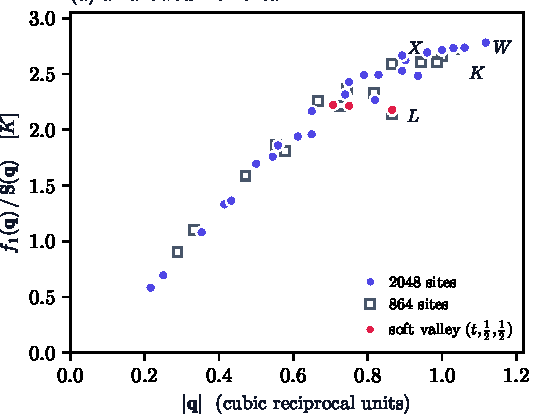
\includegraphics[width=0.55\textwidth]{fig_si_grid.pdf}
\caption{The Feynman ratio at every allowed momentum star of the
2048-site supercell (circles, statistical errors; symmetry copies
merged) with the 864-site grid overlaid (open squares). Red marks the
soft valley $(t,\frac12,\frac12)$. This is the complete data set
behind the zone-boundary comparison of Fig.~4(a) of the main text: no
path or interpolation is involved, and each value is a true eigenmode
weight of its torus.}
\label{fig:sigrid}
\end{figure}
% ================================================================

At the principal zone-boundary momenta the Feynman ratios are
\begin{center}
\begin{tabular}{lrr}
\hline\hline
&864&2048\\
\hline
$L$&$2.142(10)$&$2.179(19)$\\
$X$&$2.660(10)$&$2.713(21)$\\
$W$&---&$2.781(10)$\\
$K$&---&$2.718(20)$\\
$U$&---&$2.736(11)$\\
\hline\hline
\end{tabular}
\end{center}

The $L$ value shifts by only $1.7\%$ from 864 to 2048 sites and
remains $20$--$25\%$ below the other principal zone-boundary
momenta.

Along the radial $[111]$ direction the centroid rises monotonically
toward $L$.
On the $8^3$ cell the sequence is approximately
\begin{equation}
0.60,\quad1.36,\quad1.97,\quad2.18
\end{equation}
at the allowed momenta
\begin{equation}
\frac{k}{8}(1,1,1).
\end{equation}

Thus the centroid does not possess a helium-style radial dip.
Instead, the soft structure is a minimum within the zone-boundary
landscape.

Representative nearby values are
\begin{align}
\frac{f_1}{S}
\left(
\frac14,\frac12,\frac12
\right)
&=
2.216(5),\\
\frac{f_1}{S}
\left(
\frac38,\frac38,\frac58
\right)
&=
2.265(5),\\
\frac{f_1}{S}
\left(
\frac14,\frac12,\frac34
\right)
&=
2.484(5).
\end{align}
The result is a shallow valley extending away from $L$ rather than an
isolated point.

% ================================================================
\section{Experimental interpretation}
\label{sec:experiment}
% ================================================================

The calculation does not imply that every zone-boundary feature of a
microscopic quantum-spin-ice material must coincide quantitatively
with the low $L$ level of the pure ring model.
Longer ring exchanges, virtual spinons, further microscopic
interactions, disorder, and the material-specific magnetic moment
operator can modify the spectrum.

The calculation instead demonstrates that the minimal compact gauge
Hamiltonian can itself redistribute a large fraction of the
finite-momentum $S^z$ spectral weight without leaving the deconfined
ice manifold.

A useful experimental pattern to search for is therefore the
following:
a response that is dominated by a single photon-like feature near the
zone center need not remain single-mode at the zone boundary.
Along $[111]$, substantial spectral weight may transfer into a lower
feature while a weaker higher-energy feature remains near the
continuation of the long-wavelength photon.

The exact intensity ratio is not universal.
The physical neutron response coherently combines sublattice
amplitudes before taking the squared modulus.
The local easy axes and $g$ tensor can therefore reweight the two
branches differently and may enhance or suppress a particular feature
in a given scattering geometry.

A finite cluster also produces discrete poles where the thermodynamic
system may instead show a peak plus continuum.
The robust experimental prediction of the minimal model is therefore
\emph{redistribution and reconstruction of finite-momentum spectral
weight}, not a universal number of poles or a universal low/high
intensity ratio.

% ================================================================
\section{Scope and limitations}
\label{sec:limitations}
% ================================================================

The results establish the following directly:
\begin{enumerate}
\item
a dominant reconstructed $S^z$ level exists on all four finite
clusters from 48 to 96 sites;

\item
its weight fraction and scale-free branch ratio are stable across
those clusters;

\item
an RK flippability derivative provides an independent microscopic
fingerprint of the reconstructing momentum class;

\item
the ground-state Feynman ratio discriminates the reconstructing and
nonreconstructing classes available on the finite clusters;

\item
GFMC establishes the large-system momentum dependence of the
corresponding spectral centroid up to 2048 sites.
\end{enumerate}

Several statements remain beyond the calculation.

First, the sharpness of the reconstructed level is established only
through 96 spins.
GFMC determines ground-state quantities and therefore the spectral
centroid, not the thermodynamic linewidth.
The finite-size pole could broaden into a narrow continuum in the
thermodynamic limit.

Second, Eq.~(\ref{eq:ring_supp}) is the pure ring Hamiltonian in the
charge-free ice manifold.
Electric charges are absent by construction.
Longer ring exchanges, virtual spinon processes, and other microscopic
terms generated in a full spin Hamiltonian are outside the present
calculation.
The survival and quantitative position of the reconstructed branch
under such perturbations remain open.

Third, the calculated observable is the sublattice-summed pseudospin
response rather than the coherent material-specific neutron cross
section.
The experimental visibility of the low branch should therefore be
tested by applying the appropriate magnetic projection for a chosen
material.

% ================================================================
\section{Additional spectra}
% ================================================================

\begin{figure}[t]
\centering
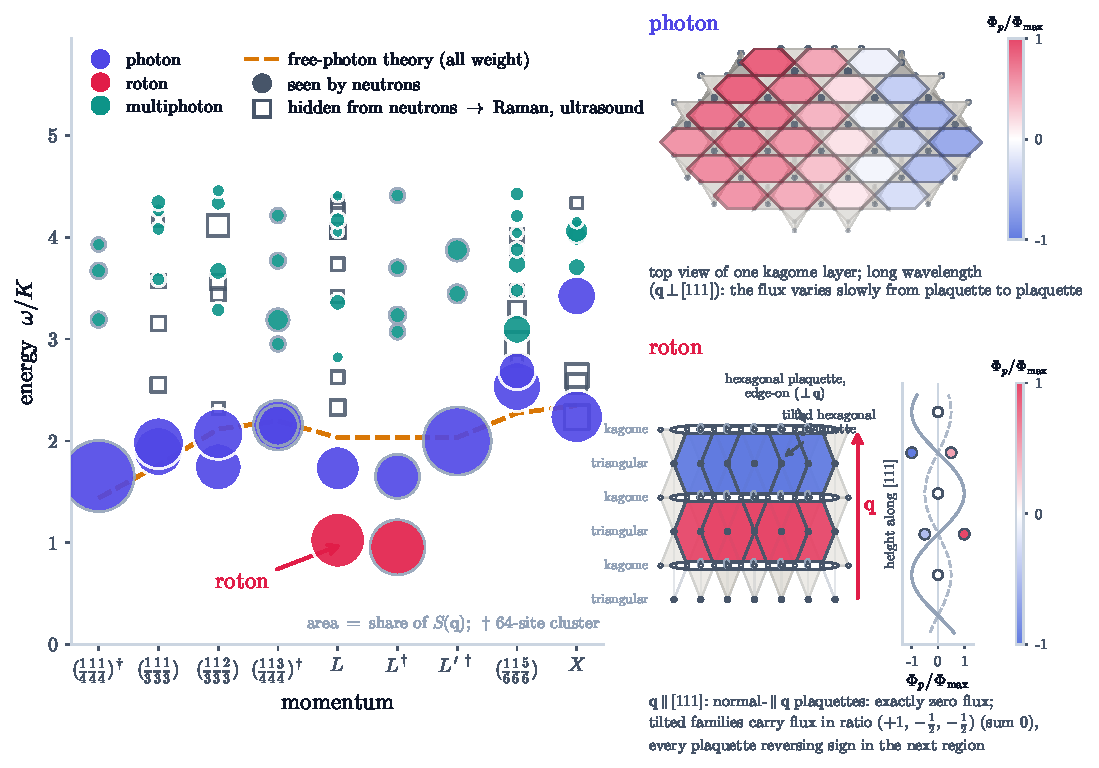
\includegraphics[width=0.93\textwidth]{fig_hero.pdf}
\caption{
Full operator-resolved finite-size spectrum and state diagnostics.
Marker area represents the sublattice-summed $S^z$ spectral weight.
}
\label{fig:hero_supp}
\end{figure}

\begin{figure}[t]
\centering

\includegraphics[width=0.93\textwidth]{fig_dssf.pdf}
\caption{
Resolved $\Szz(\bq,\omega)$ near the reconstructed region.
The broadening is used only for display; quoted energies and weights
are extracted from the discrete poles.
}
\label{fig:dssf_supp}
\end{figure}

\begin{figure}[t]
\centering
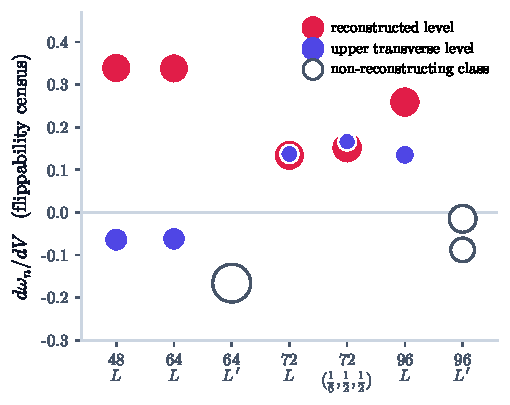
\includegraphics[width=0.93\textwidth]{fig_mechanism.pdf}
\caption{
Full RK deformation and flippability diagnostics for the finite-size
states.
}
\label{fig:rk_supp}
\end{figure}

\begin{figure}[t]
\centering
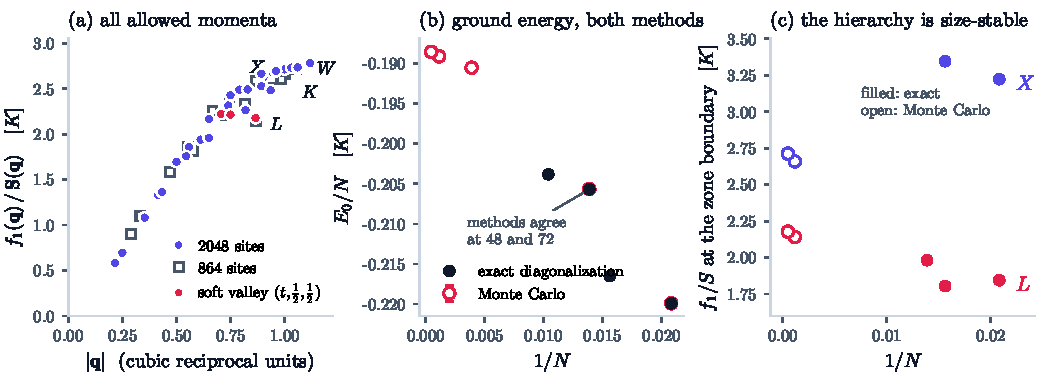
\includegraphics[width=0.93\textwidth]{fig_thermo.pdf}
\caption{
Complete large-system GFMC diagnostics and Feynman-ratio landscape.
}
\label{fig:thermo_supp}
\end{figure}

\begin{acknowledgments}
We thank the Digital Research Alliance of Canada for computational
resources.
The complete set of scripts generating every number, numerical gate,
and figure reported in this work is included with the submission.
\end{acknowledgments}

\bibliographystyle{apsrev4-2}
\bibliography{refs}

\end{document}